% !TEX program = xelatex
\documentclass[12pt,a4paper]{article}

% =========================================
% Packages
% =========================================
\usepackage{geometry}
\geometry{a4paper, margin=2.5cm}
\usepackage{graphicx}
\usepackage{amsmath}
\usepackage{float}
\usepackage{fancyhdr}
\usepackage[svgnames]{xcolor}

% رفع خطای ارتفاع هدر
\setlength{\headheight}{32pt}

% تنظیمات لینک‌ها
\usepackage[hidelinks]{hyperref}
\hypersetup{
	colorlinks=true,
	linkcolor=NavyBlue,
	filecolor=Magenta,
	urlcolor=DarkBlue,
	pdftitle={سیستم آرکید بازی‌لند},
	pdfauthor={علیرضا زارع‌بیدکی},
}

% تنظیمات کدنویسی
\usepackage{listings}

% =========================================
% Code Listing Configuration
% =========================================
\definecolor{codegreen}{rgb}{0,0.6,0}
\definecolor{codegray}{rgb}{0.5,0.5,0.5}
\definecolor{codepurple}{rgb}{0.58,0,0.82}
\definecolor{backcolour}{rgb}{0.96,0.96,0.96}
\definecolor{codeblue}{rgb}{0.13,0.13,1}

\lstdefinestyle{mystyle}{
	backgroundcolor=\color{backcolour},
	commentstyle=\color{codegreen},
	keywordstyle=\color{codeblue}\bfseries,
	numberstyle=\tiny\color{codegray},
	stringstyle=\color{codepurple},
	basicstyle=\ttfamily\footnotesize,
	breakatwhitespace=false,
	breaklines=true,
	captionpos=b,
	keepspaces=true,
	numbers=left,
	numbersep=5pt,
	showspaces=false,
	showstringspaces=false,
	showtabs=false,
	tabsize=4,
	frame=single,
	rulecolor=\color{gray!30},
	escapechar=@,
	literate=
	{$}{{\textcolor{codeblue}{\$}}}1
	{^}{{\textasciicircum}}1
}

\lstset{style=mystyle,
	literate=
	{│}{|}1
	{├}{|--}3
	{─}{--}2
	{└}{|__}3
	{$}{{\textcolor{codeblue}{\$}}}1
}

% تعریف زبان JavaScript
\lstdefinelanguage{JavaScript}{
	keywords={break, case, catch, continue, debugger, default, delete,
		do, else, finally, for, function, if, in, instanceof, new, return,
		switch, this, throw, try, typeof, var, void, while, with, let, const, await, async},
	sensitive=true,
	comment=[l]{//},
	morecomment=[s]{/*}{*/},
	morestring=[b]',
	morestring=[b]"
}

% تعریف زبان CSS
\lstdefinelanguage{CSS}{
	keywords={color,background,margin,padding,font,weight,display,position,top,left,right,bottom,list,style,border,size,white,space,min,width,transition,transform,transition-property,transition-duration,transition-timing-function,perspective,transform-style,rotateX,text-shadow},
	sensitive=true,
	morecomment=[l]{//},
	morecomment=[s]{/*}{*/},
	morestring=[b]',
	morestring=[b]",
	alsoletter={-}
}

% تعریف زبان JSON
\lstdefinelanguage{JSON}{
	basicstyle=\ttfamily\footnotesize,
	string=[s]{"}{"},
	stringstyle=\color{codepurple},
	comment=[l]{:},
	commentstyle=\color{black},
}

% =========================================
% Persian Support (Must be last)
% =========================================
\usepackage{xepersian}
% تنظیم فونت‌ها (حتماً فونت‌ها در کنار فایل تکس باشند)
\settextfont[Scale=1.1, Path=./]{XB Niloofar.ttf}
\setlatintextfont[Path=./]{times.ttf}
\setdigitfont[Path=./]{XB Niloofar.ttf}

% تنظیم فاصله بین پاراگراف‌ها
\setlength{\parskip}{0.5em}
\setlength{\parindent}{0pt}

% =========================================
% Header and Footer
% =========================================
\pagestyle{fancy}
\fancyhf{}
\fancyhead[R]{\thepage}
\fancyhead[L]{سیستم آرکید بازی‌لند}
\renewcommand{\headrulewidth}{1pt}

% =========================================
% Title Information
% =========================================
\title{\textbf{طراحی و پیاده‌سازی سیستم آرکید وب‌محور بازی‌لند:\\
		معماری \lr{CGI}، مدیریت \lr{Stateless} و تجربه کاربری نوستالژیک}}

\author{علیرضا زارع‌بیدکی\\
	\lr{Alireza ZareBidoki}\\
	\small \lr{alireza@zarebidoki.com}\\
	\small \url{https://github.com/alireza-zarebidoki}}

\date{\texorpdfstring{۶ دی ۱۴۰۴ -- \lr{December 26, 2025}}{6 Dey 1404 - December 26, 2025}}

% =========================================
% Document Start
% =========================================
\begin{document}
	
	\maketitle
	\thispagestyle{empty}
	
	\begin{abstract}
		\noindent\textbf{نسخه زنده:} \url{https://baziland.zarebidoki.com/}
		
		\vspace{0.3cm}
		
		این مقاله به معرفی و تحلیل معماری سیستم آرکید بازی‌لند \lr{(BAZI LAND Arcade System)} می‌پردازد که یک پلتفرم وب‌محور برای اجرای بازی‌های آرکیدی کلاسیک با رویکرد نوستالژیک است.
		این سیستم شامل ۷ بازی تعاملی (حدس عدد، دوز محدود، سنگ کاغذ قیچی پنج حرکتی، حلقه آویز، فیبوناچی ۲۰۴۸، شطرنج تغییریافته، و چکرز) است که با استفاده از معماری \lr{CGI} در زبان \lr{C} پیاده‌سازی شده و با رابط کاربری \lr{JavaScript} خالص و \lr{CSS3} با افکت‌های سه‌بعدی و نئونی ارائه می‌شود.
		سیستم دارای معماری \lr{stateless}، سیستم احراز هویت مبتنی بر سشن، سیستم اقتصادی سکه‌محور، و پنل مدیریتی است.
		در این مقاله به تحلیل معماری، تصمیمات طراحی، جزئیات پیاده‌سازی، چالش‌های امنیتی و فنی، و راهکارهای آینده پرداخته می‌شود.
		
		\textbf{کلمات کلیدی:}
		سیستم آرکید، \lr{CGI}، معماری \lr{Stateless}، \lr{Vanilla JavaScript}، احراز هویت، طراحی نوستالژیک، بازی‌های وب
		
		\vspace{0.5cm}
		\hrule
		\vspace{0.5cm}
		
		\begin{latin}
			\textbf{Abstract:}\\
			This paper presents BAZI LAND, a web-based arcade gaming platform featuring 7 interactive games implemented using CGI architecture in C, with a nostalgic user interface built with vanilla JavaScript and CSS3 including 3D and neon effects.
			The system employs stateless architecture, session-based authentication, coin-based economy, and administrative management panel.
			We analyze the architecture, design decisions, implementation details, challenges, and future directions.
		\end{latin}
	\end{abstract}
	
	\newpage
	\tableofcontents
	\newpage
	
	\section{مقدمه}
	
	\subsection{نگاهی کلی}
	بازی‌لند یک سیستم آرکید وب‌محور است که با هدف بازآفرینی تجربه کابینت‌های آرکیدی دهه ۱۹۸۰ و ۱۹۹۰ میلادی در محیط مرورگر طراحی و پیاده‌سازی شده است.
	این سیستم ترکیبی از تکنولوژی‌های سنتی (\lr{CGI with C}) و مدرن (\lr{HTML5, CSS3, Vanilla JavaScript}) را برای ایجاد یک تجربه یکپارچه و نوستالژیک به کار می‌گیرد.
	
	\subsection{انگیزه و اهداف}
	اهداف اصلی این پروژه عبارتند از:
	
	\begin{itemize}
		\item \textbf{بازآفرینی تجربه آرکید کلاسیک:} شبیه‌سازی کامل یک کابینت آرکید از جمله ظاهر بصری، سیستم سکه، و رابط کاربری مشابه.
		\item \textbf{یادگیری معماری \lr{CGI}:} بررسی و پیاده‌سازی معماری \lr{Common Gateway Interface} که یکی از اولین و بنیادی‌ترین روش‌های ایجاد وب اپلیکیشن‌های پویا است.
		\item \textbf{طراحی \lr{Stateless}:} استفاده از معماری بدون وضعیت که در آن تمام \lr{state} بازی در \lr{URL parameters} انتقال می‌یابد.
		\item \textbf{توسعه بدون \lr{Framework}:} استفاده از \lr{Vanilla JavaScript} به جای کتابخانه‌های سنگین مانند \lr{React} یا \lr{Vue} برای درک عمیق‌تر مفاهیم بنیادی وب.
		\item \textbf{تجربه کاربری منحصر به فرد:} ایجاد یک رابط کاربری با افکت‌های نئونی، سه‌بعدی، و انیمیشن‌های پیچیده که حس استفاده از یک دستگاه آرکید واقعی را منتقل کند.
	\end{itemize}
	
	\subsection{دامنه کاربرد}
	این سیستم برای موارد زیر قابل استفاده است:
	
	\begin{itemize}
		\item سرگرمی و بازی‌های کوتاه‌مدت
		\item آموزش برنامه‌نویسی وب و معماری \lr{CGI}
		\item مطالعه موردی در طراحی سیستم‌های \lr{stateless}
		\item پلتفرم نمونه برای توسعه‌دهندگان
	\end{itemize}
	
	\section{پیشینه و مفاهیم}
	
	\subsection{سیستم‌های آرکید کلاسیک}
	دستگاه‌های آرکید در دهه‌های ۱۹۷۰ تا ۱۹۹۰ میلادی نقش مهمی در صنعت بازی داشتند.
	این دستگاه‌ها معمولاً دارای یک کابینت چوبی یا فلزی، مانیتور \lr{CRT}، جویستیک، دکمه‌های رنگی، و سیستم سکه بودند.
	بازی‌لند قصد دارد تمام این عناصر را در یک محیط وب شبیه‌سازی کند.
	
	\subsection{معماری \lr{Common Gateway Interface (CGI)}}
	\lr{CGI} یک استاندارد برای اجرای برنامه‌های خارجی توسط سرور وب است که در سال ۱۹۹۳ معرفی شد.
	در این معماری:
	
	\begin{enumerate}
		\item مرورگر یک درخواست \lr{HTTP} به سرور ارسال می‌کند.
		\item سرور یک \lr{process} جدید برای اجرای برنامه \lr{CGI} ایجاد می‌کند.
		\item برنامه \lr{CGI} خروجی \lr{HTML} تولید می‌کند.
		\item سرور خروجی را به مرورگر برمی‌گرداند.
		\item \lr{Process} پایان می‌یابد.
	\end{enumerate}
	
	مزایای \lr{CGI}:
	\begin{itemize}
		\item سادگی و عدم نیاز به \lr{runtime} سنگین
		\item هر درخواست مستقل است
		\item امکان استفاده از هر زبان برنامه‌نویسی
	\end{itemize}
	
	معایب \lr{CGI}:
	\begin{itemize}
		\item ایجاد \lr{process} جدید برای هر درخواست (\lr{overhead})
		\item عدم امکان حفظ \lr{state} بین درخواست‌ها
		\item مقیاس‌پذیری محدود برای \lr{traffic} بالا
	\end{itemize}
	
	\subsection{معماری \lr{Stateless}}
	در معماری \lr{stateless}، سرور هیچ اطلاعاتی از وضعیت قبلی کلاینت را حفظ نمی‌کند.
	تمام اطلاعات لازم برای پردازش درخواست باید در خود درخواست موجود باشد.
	در بازی‌لند، تمام وضعیت بازی در \lr{URL parameters} قرار می‌گیرد.
	
	مثال:
	\begin{latin}
		\begin{verbatim}
			/cgi-bin/tictactoe_limited.cgi?p1=0,4,8&p2=1,5&turn=1&move=2
		\end{verbatim}
	\end{latin}
	
	در این \lr{URL}:
	\begin{itemize}
		\item \texttt{p1=0,4,8}: مهره‌های بازیکن ۱ در خانه‌های ۰، ۴، ۸
		\item \texttt{p2=1,5}: مهره‌های بازیکن ۲ در خانه‌های ۱، ۵
		\item \texttt{turn=1}: نوبت بازیکن ۱
		\item \texttt{move=2}: حرکت بعدی به خانه ۲
	\end{itemize}
	
	\newpage
	\section{معماری سیستم}
	
	\subsection{نمای کلی معماری}
	
	سیستم بازی‌لند از معماری سه‌لایه استفاده می‌کند:
	
	\begin{enumerate}
		\item \textbf{لایه رابط کاربری (Frontend):} \lr{HTML5, CSS3, Vanilla JavaScript}
		\item \textbf{لایه منطق (Backend):} برنامه‌های \lr{CGI} نوشته شده با \lr{C}
		\item \textbf{لایه داده (Data Layer):} فایل‌های \lr{JSON} برای ذخیره‌سازی
	\end{enumerate}
	
	\begin{figure}[H]
		\centering
		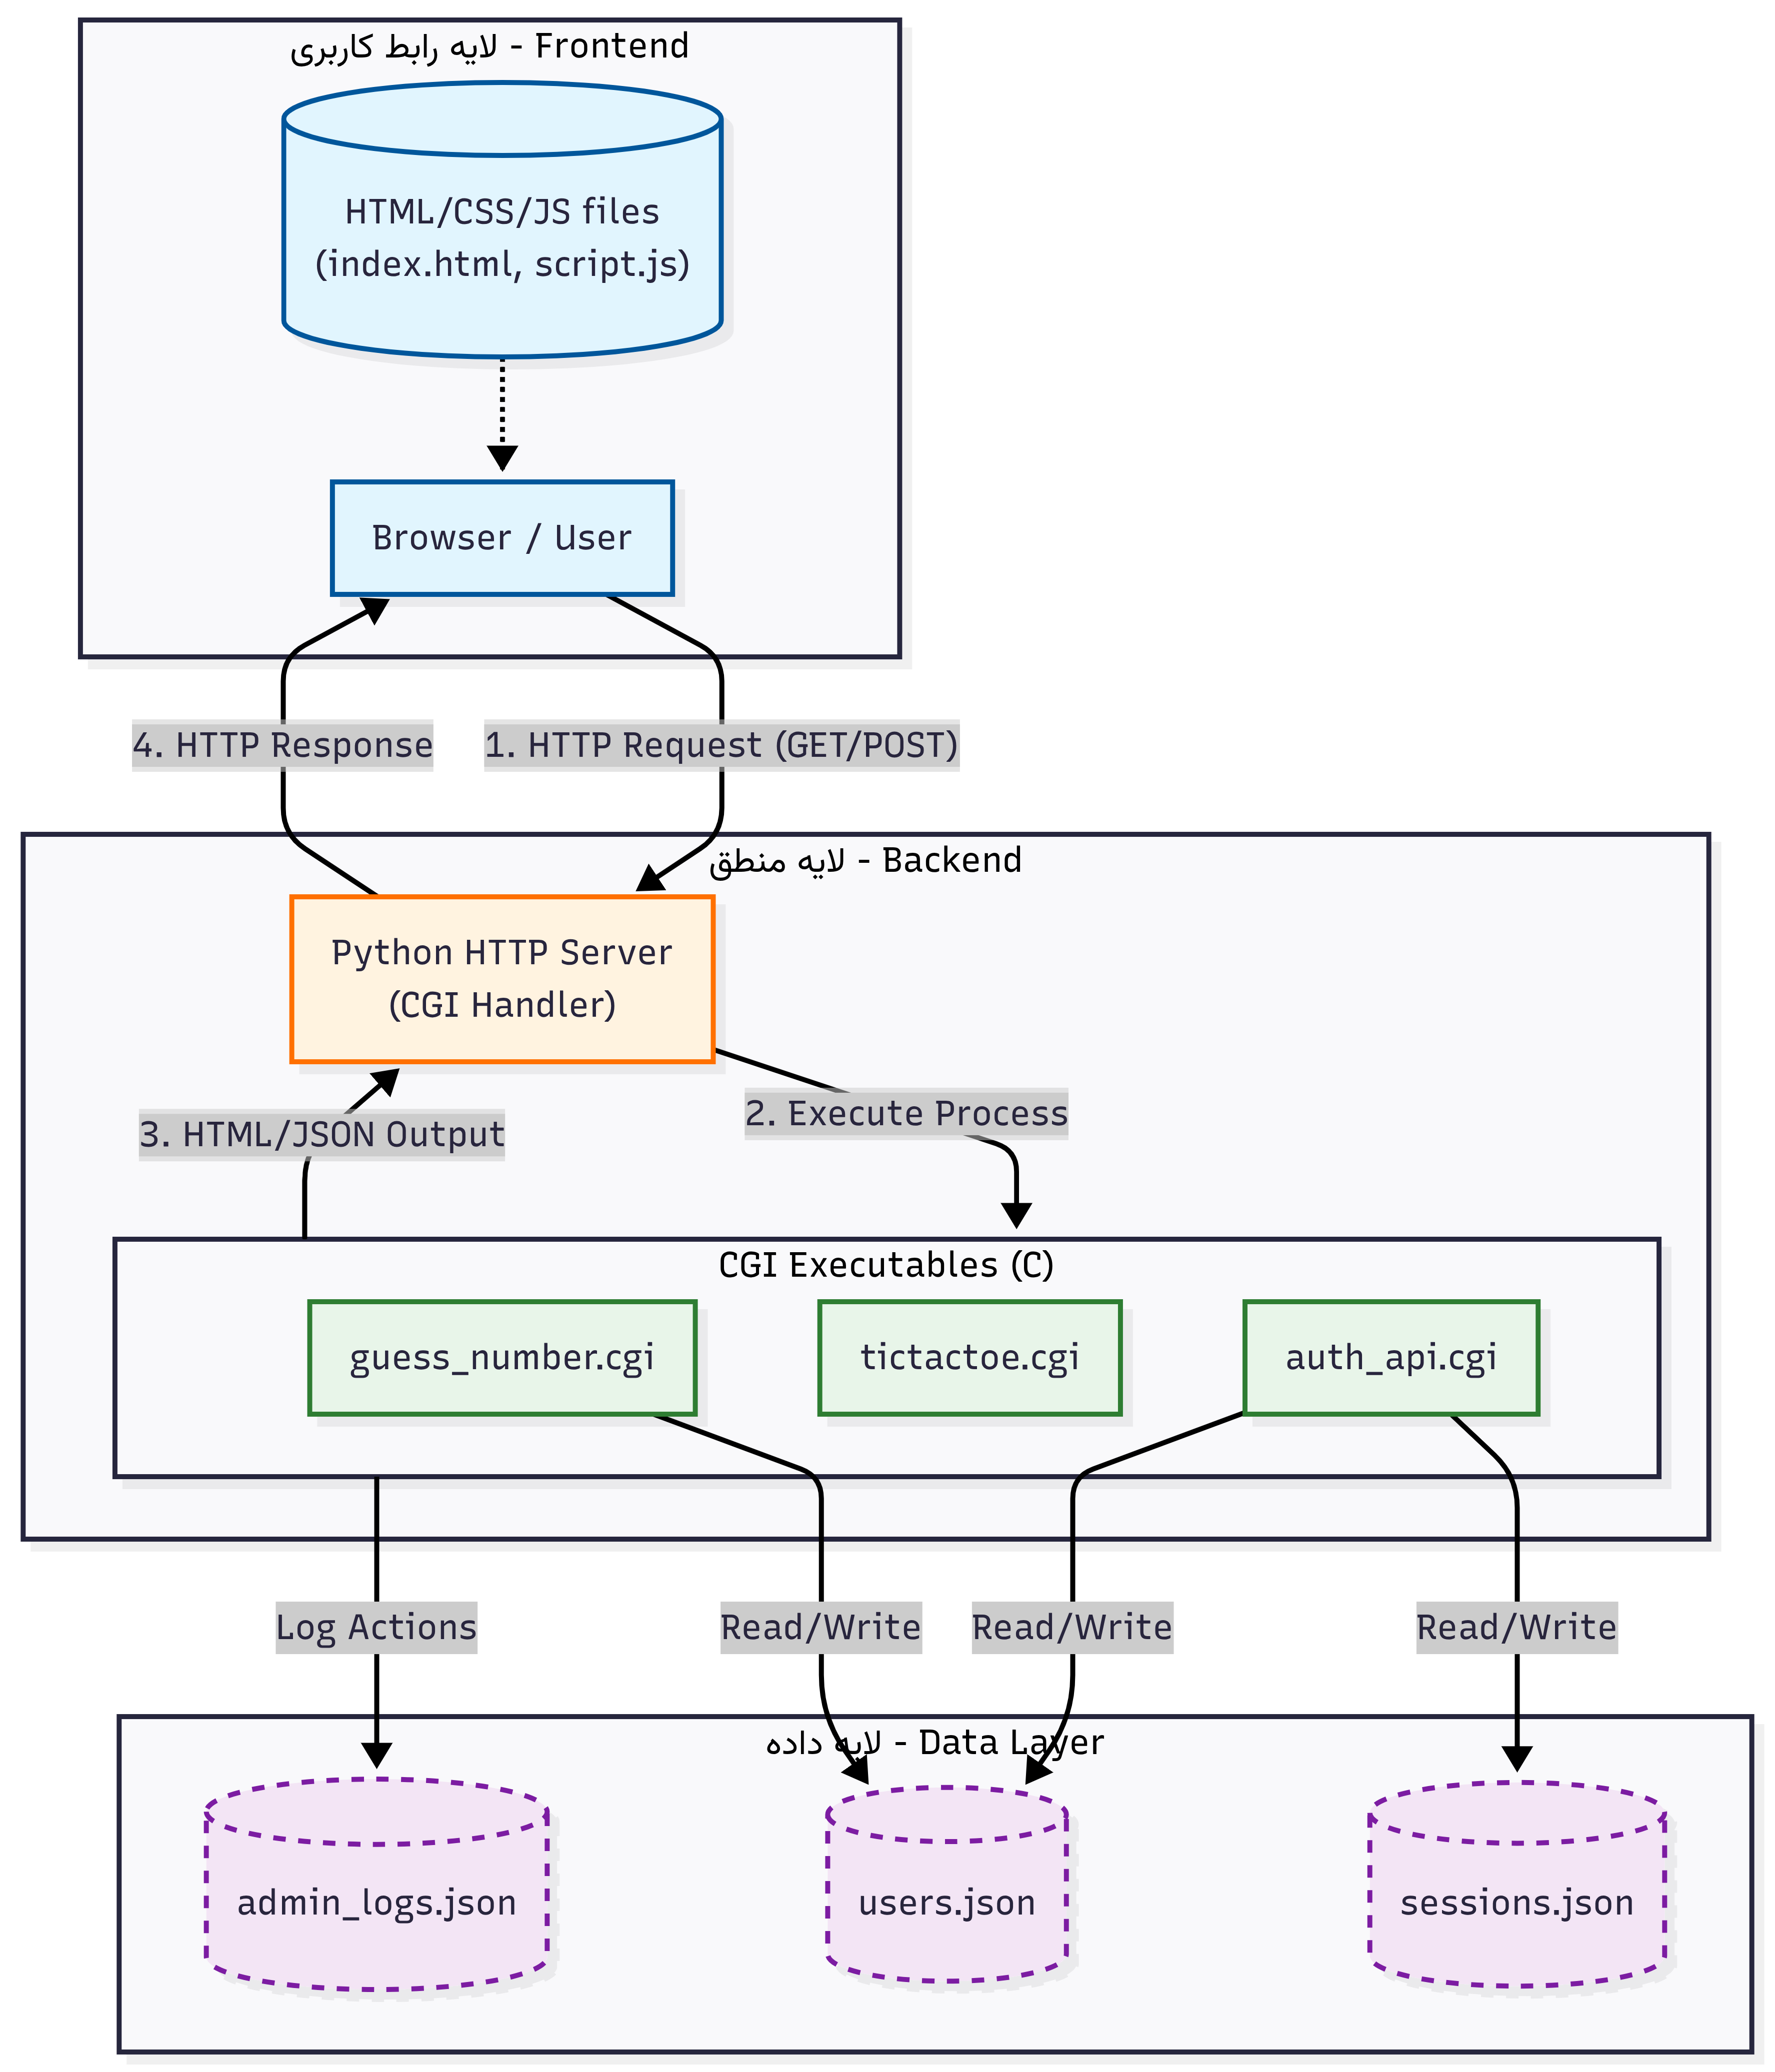
\includegraphics[width=1.0\linewidth]{architecture_diagram.png}
		\caption{نمای کلی معماری سیستم بازی‌لند و جریان داده بین لایه‌ها}
		\label{fig:architecture}
	\end{figure}
	
	\subsection{ساختار پروژه}
	
	ساختار پوشه‌های پروژه به شرح زیر است:
	
\begin{latin}
	\begin{lstlisting}[language=bash, caption=ساختار پوشه‌ها]
		arcade-system/
		|-- index.html              # Main page
		|-- style.css               # Styles (1128 lines)
		|-- script.js               # Frontend logic (1353 lines)
		|-- auth.js                 # Auth module (328 lines)
		|-- Makefile                # Build system
		|
		|-- src/
		|   |-- common/
		|   |   |-- c_utils.h       # CGI helper functions
		|   |   |__ c_utils.c
		|   |
		|   |__ games/
		|       |-- guess_number.c
		|       |-- tictactoe_limited.c
		|       |-- rps_5move.c
		|       |-- hangman_battle.c
		|       |-- fibonacci_2048.c
		|       |-- chess/          # Chess (4 files)
		|       |__ checkers/       # Checkers (4 files)
		|
		|-- cgi-bin/                # Compiled CGI files
		|   |-- guess_number.cgi
		|   |-- tictactoe_limited.cgi
		|   |__ ...
		|
		|__ data/                   # JSON files
		|-- users.json
		|-- sessions.json
		|-- admin.json
		|__ admin_logs.json
	\end{lstlisting}
\end{latin}
	
	\subsection{جریان اجرا}
	
	جریان کلی از انتخاب بازی تا اجرا به شرح زیر است:
	
	\begin{enumerate}
		\item کاربر صفحه اصلی را باز می‌کند (\texttt{index.html}).
		\item \lr{JavaScript} کاروسل بازی‌ها را نمایش می‌دهد.
		\item کاربر یک بازی را انتخاب می‌کند.
		\item سیستم احراز هویت بررسی می‌شود (\texttt{auth.js}).
		\item موجودی سکه کاربر بررسی می‌شود.
		\item در صورت کافی بودن، سکه کسر می‌شود.
		\item یک \texttt{iframe} با \lr{URL} مربوط به بازی ساخته می‌شود.
		\item سرور \lr{Python} درخواست را به \lr{CGI} مربوطه ارسال می‌کند.
		\item برنامه \lr{CGI} اجرا شده و \lr{HTML} تولید می‌کند.
		\item مرورگر \lr{HTML} را در \texttt{iframe} نمایش می‌دهد.
		\item کاربر با بازی تعامل می‌کند و \lr{CGI} مجدداً با \lr{state} جدید اجرا می‌شود.
	\end{enumerate}
	
	\newpage
	\section{بازی‌های موجود}
	
	سیستم بازی‌لند دارای ۷ بازی است که هر کدام به صورت مستقل پیاده‌سازی شده‌اند.
	
	\subsection{حدس عدد (\lr{Guess Number})}
	\textbf{توضیح:} بازیکن باید عدد تصادفی بین ۱ تا ۱۰۰ را حدس بزند.
	\textbf{سطوح دشواری:}
	\begin{itemize}
		\item \textbf{آسان:} ۱۰ تلاش، راهنمایی دقیق
		\item \textbf{متوسط:} ۷ تلاش، راهنمایی کلی
		\item \textbf{سخت:} ۵ تلاش، راهنمایی مبهم
	\end{itemize}
	\textbf{قیمت:} ۳ سکه\\
	\textbf{پاداش:} ۵ سکه
	
	\subsection{دوز محدود (\lr{Tic-Tac-Toe Limited})}
	\textbf{توضیح:} نسخه تغییریافته دوز با محدودیت ۳ مهره برای هر بازیکن.
	\textbf{قانون خاص:} وقتی مهره چهارم گذاشته می‌شود، قدیمی‌ترین مهره به صورت \lr{FIFO} حذف می‌شود.
	\textbf{منطق \lr{FIFO}:}
	\begin{latin}
		\begin{lstlisting}[language=C, caption=الگوریتم FIFO در دوز محدود]
			if (count(player_moves) >= 3) {
				remove_oldest_move(player_moves);
			}
			add_new_move(player_moves, move);
		\end{lstlisting}
	\end{latin}
	
	\textbf{قیمت:} ۵ سکه\\
	\textbf{پاداش:} ۸ سکه
	
	\subsection{سنگ کاغذ قیچی++ (\lr{RPS 5-Move})}
	\textbf{توضیح:} نسخه ۵ حرکتی از سریال \lr{Big Bang Theory}.
	\textbf{حرکات:}
	\begin{itemize}
		\item \lr{Rock} (سنگ)
		\item \lr{Paper} (کاغذ)
		\item \lr{Scissors} (قیچی)
		\item \lr{Lizard} (مارمولک)
		\item \lr{Spock} (اسپاک)
	\end{itemize}
	
	\textbf{قوانین:}
	\begin{itemize}
		\item سنگ $>$ قیچی، مارمولک
		\item کاغذ $>$ سنگ، اسپاک
		\item قیچی $>$ کاغذ، مارمولک
		\item مارمولک $>$ کاغذ، اسپاک
		\item اسپاک $>$ سنگ، قیچی
	\end{itemize}
	
	\textbf{قیمت:} ۴ سکه\\
	\textbf{پاداش:} ۶ سکه
	
	\subsection{حلقه آویز (\lr{Hangman Battle})}
	\textbf{توضیح:} دو بازیکن هم‌زمان در دو بازی حلقه آویز شرکت می‌کنند.
	\textbf{حالت‌ها:}
	\begin{itemize}
		\item \lr{Player vs Player}
		\item \lr{Player vs Bot}
	\end{itemize}
	
	\textbf{استراتژی \lr{Bot}:} بر اساس فرکانس حروف در زبان انگلیسی:
	\begin{latin}
		\begin{verbatim}
			ETAOINSHRDLCUMWFGYPBVKJXQZ
		\end{verbatim}
	\end{latin}
	
	\textbf{قیمت:} ۶ سکه\\
	\textbf{پاداش:} ۱۰ سکه
	
	\subsection{فیبوناچی ۲۰۴۸}
	\textbf{توضیح:} نسخه تغییریافته ۲۰۴۸ با قوانین دنباله فیبوناچی.
	\textbf{قانون اصلی:} فقط اعداد مجاور در دنباله فیبوناچی می‌توانند ترکیب شوند:
	
	$$
	1 + 1 = 2, \quad 1 + 2 = 3, \quad 2 + 3 = 5, \quad 3 + 5 = 8, \quad \ldots
	$$
	
	\textbf{اندازه‌های صفحه:} $4 \times 4$، $5 \times 5$، $6 \times 6$
	
	\textbf{قیمت:} ۷ سکه\\
	\textbf{پاداش:} ۱۲ سکه
	
	\subsection{شطرنج تغییریافته}
	\textbf{توضیح:} شطرنج با ۳ مهره جدید.
	\textbf{مهره‌های جدید:}
	\begin{itemize}
		\item \textbf{اژدها (\lr{Dragon}):} جایگزین اسب. ترکیب حرکت اسب + شاه (۱۶ حرکت ممکن).
		\item \textbf{دزد (\lr{Thief}):} جایگزین فیل. فیل با قابلیت پرش از یک مانع.
		\item \textbf{گریفین (\lr{Gryphon}):} جایگزین رخ. یک خانه مورب + سپس حرکت رخ.
	\end{itemize}
	
	\textbf{تایمر:} هر بازیکن ۱۰ دقیقه\\
	\textbf{قیمت:} ۱۰ سکه\\
	\textbf{پاداش:} ۲۰ سکه
	
	\subsection{چکرز (\lr{Checkers})}
	\textbf{توضیح:} بازی چکرز کلاسیک با قوانین استاندارد.
	\textbf{قوانین اصلی:}
	\begin{itemize}
		\item حرکت مهره: یک خانه مورب به جلو
		\item پرش: خوردن مهره حریف
		\item پرش زنجیره‌ای: اگر بعد از پرش، پرش دیگری ممکن باشد
		\item \lr{King} شدن: رسیدن به انتهای صفحه
	\end{itemize}
	\textbf{قیمت:} ۸ سکه\\
	\textbf{پاداش:} ۱۵ سکه
	
	\newpage
	\section{جزئیات پیاده‌سازی}
	
	\subsection{Backend: توابع کمکی \lr{CGI}}
	
	تمام بازی‌های \lr{CGI} از توابع مشترکی استفاده می‌کنند که در \texttt{c\_utils.h/c} تعریف شده‌اند.
	
	\subsubsection{تابع \texttt{print\_header()}}
	این تابع \lr{HTTP header} لازم برای \lr{CGI} را چاپ می‌کند:
	
	\begin{latin}
		\begin{lstlisting}[language=C, caption=تابع print\_header]
			void print_header() {
				printf("Content-Type: text/html; charset=UTF-8\n\n");
			}
		\end{lstlisting}
	\end{latin}
	
	\subsubsection{تابع \texttt{get\_param()}}
	این تابع مقدار یک پارامتر از \texttt{QUERY\_STRING} را استخراج می‌کند:
	
	\begin{latin}
		\begin{lstlisting}[language=C, caption=تابع get\_param]
			char* get_param(const char* name) {
				char *query = getenv("QUERY_STRING");
				if (!query) return NULL;
				
				// Parse query string
				char *token = strtok(query, "&");
				while (token) {
					char *eq = strchr(token, '=');
					if (eq) {
						*eq = '\0';
						if (strcmp(token, name) == 0) {
							char *value = eq + 1;
							char *decoded = malloc(MAX_PARAM_LEN);
							url_decode(decoded, value);
							return decoded;
						}
					}
					token = strtok(NULL, "&");
				}
				return NULL;
			}
		\end{lstlisting}
	\end{latin}
	
	\subsubsection{تابع \texttt{url\_decode()}}
	این تابع \lr{URL encoding} را به رشته عادی تبدیل می‌کند:
	
	\begin{latin}
		\begin{lstlisting}[language=C, caption=تابع url\_decode]
			void url_decode(char* dst, const char* src) {
				while (*src) {
					if (*src == '%') {
						int value;
						sscanf(src + 1, "%2x", &value);
						*dst++ = (char)value;
						src += 3;
					} else if (*src == '+') {
						*dst++ = ' ';
						src++;
					} else {
						*dst++ = *src++;
					}
				}
				*dst = '\0';
			}
		\end{lstlisting}
	\end{latin}
	
	\subsection{Frontend: معماری \lr{JavaScript}}
	رابط کاربری با استفاده از \lr{Vanilla JavaScript} پیاده‌سازی شده است.
	
	\subsubsection{کاروسل بازی‌ها}
	کاروسل بازی‌ها با استفاده از \texttt{transform: translateX()} پیاده‌سازی شده:
	
	\begin{latin}
		\begin{lstlisting}[language=JavaScript, caption=کاروسل بازی‌ها]
			function updateCarousel() {
				const itemWidth = 120;  // px
				const gap = 20;         // px
				const offset = -(currentIndex * (itemWidth + gap));
				carousel.style.transform = `translateX(${offset}px)`;
				updateActiveGame();
			}
			
			function nextGame() {
				currentIndex = (currentIndex + 1) % gameItems.length;
				updateCarousel();
			}
			
			function prevGame() {
				currentIndex = (currentIndex - 1 + gameItems.length)
				% gameItems.length;
				updateCarousel();
			}
		\end{lstlisting}
	\end{latin}
	
	فرمول ریاضی موقعیت کاروسل:
	$$
	\text{Position} = -(\text{index} \times (\text{itemWidth} + \text{gap}))
	$$
	
	\subsubsection{ماژول احراز هویت}
	ماژول \texttt{auth.js} با استفاده از الگوی \lr{IIFE} پیاده‌سازی شده:
	
	\begin{latin}
		\begin{lstlisting}[language=JavaScript, caption=ماژول احراز هویت]
			const Auth = (function() {
				const API_BASE = '/cgi-bin/auth_api.cgi';
				
				// Private functions
				function saveSession(user) {
					localStorage.setItem('user', JSON.stringify(user));
					localStorage.setItem('sessionToken', user.sessionToken);
				}
				
				// Public API
				return {
					login: async function(username, password) {
						const response = await fetch(`${API_BASE}?action=login`, {
							method: 'POST',
							body: JSON.stringify({ username, password })
						});
						const data = await response.json();
						if (data.success) {
							saveSession(data.user);
						}
						return data;
					},
					
					isLoggedIn: function() {
						return localStorage.getItem('user') !== null;
					},
					
					getUser: function() {
						const userStr = localStorage.getItem('user');
						return userStr ? JSON.parse(userStr) : null;
					}
				};
			})();
		\end{lstlisting}
	\end{latin}
	
	\subsection{Frontend: افکت‌های بصری \lr{CSS}}
	
	\subsubsection{افکت نئونی (\lr{Neon Glow})}
	برای ایجاد افکت نئونی، از چندین لایه \texttt{text-shadow} استفاده می‌شود:
	
	\begin{latin}
		\begin{lstlisting}[language=CSS, caption=افکت نئونی]
			.marquee {
				color: var(--neon-green);
				text-shadow:
				0 0 5px #fff,
				0 0 10px var(--neon-green),
				0 0 20px var(--neon-green),
				0 0 40px var(--neon-green);
			}
		\end{lstlisting}
	\end{latin}
	
	\subsubsection{افکت سه‌بعدی (\lr{3D Perspective})}
	برای کنترل دک از \texttt{perspective} و \texttt{rotateX} استفاده شده:
	
	\begin{latin}
		\begin{lstlisting}[language=CSS, caption=افکت سه‌بعدی]
			.control-deck {
				perspective: 500px;
			}
			
			.deck-surface {
				transform: rotateX(20deg);
				transform-style: preserve-3d;
			}
		\end{lstlisting}
	\end{latin}
	
	\subsubsection{افکت \lr{CRT}}
	برای شبیه‌سازی مانیتور \lr{CRT}، از خطوط اسکن و شکل بیضوی استفاده شده:
	
	\begin{latin}
		\begin{lstlisting}[language=CSS, caption=افکت CRT]
			.crt-screen {
				border-radius: 80px / 30px;
				position: relative;
			}
			
			.crt-screen::before {
				content: '';
				position: absolute;
				top: 0;
				left: 0;
				width: 100%;
				height: 100%;
				background: repeating-linear-gradient(
				0deg,
				rgba(0, 0, 0, 0.15),
				rgba(0, 0, 0, 0.15) 1px,
				transparent 1px,
				transparent 2px
				);
				pointer-events: none;
			}
		\end{lstlisting}
	\end{latin}
	
	\subsection{لایه داده: \lr{JSON Files}}
	اطلاعات کاربران، سشن‌ها، و لاگ‌ها در فایل‌های \lr{JSON} ذخیره می‌شوند.
	
	\subsubsection{ساختار \texttt{users.json}}
	\begin{latin}
		\begin{lstlisting}[language=JSON, caption=ساختار users.json]
			{
				"users": [
				{
					"username": "admin",
					"password": "hashed_password",
					"coins": 1000,
					"role": "admin",
					"created_at": "2025-12-26T10:30:00Z",
					"last_login": "2025-12-26T15:20:00Z"
				}
				]
			}
		\end{lstlisting}
	\end{latin}
	
	\subsubsection{ساختار \texttt{admin\_logs.json}}
	\begin{latin}
		\begin{lstlisting}[language=JSON, caption=ساختار admin\_logs.json]
			{
				"logs": [
				{
					"id": 1,
					"username": "ali",
					"action": "subtract",
					"amount": 5,
					"reason": "Tic-Tac-Toe Limited",
					"timestamp": "2025-12-26T15:10:00Z",
					"before": 50,
					"after": 45
				}
				]
			}
		\end{lstlisting}
	\end{latin}
	
	
	\newpage
	\section{تصمیمات طراحی}
	
	\subsection{انتخاب \lr{C} برای \lr{Backend}}
	\textbf{دلایل:}
	\begin{itemize}
		\item \textbf{عملکرد:} کامپایل شده و سریع
		\item \textbf{یادگیری:} تجربه کار با \lr{memory management} و \lr{pointers}
		\item \textbf{چالش:} سخت‌تر از \lr{PHP} یا \lr{Node.js}
		\item \textbf{سبک:} بدون نیاز به \lr{runtime} سنگین
	\end{itemize}
	
	\textbf{معایب:}
	\begin{itemize}
		\item \lr{Debug} سخت‌تر
		\item مدیریت \lr{string} پیچیده
		\item نیاز به \lr{manual memory management}
	\end{itemize}
	
	\subsection{انتخاب \lr{CGI} به جای \lr{FastCGI}}
	\textbf{دلایل:}
	\begin{itemize}
		\item سادگی: نیاز به \lr{setup} کمتر
		\item آموزشی: درک بهتر از \lr{HTTP protocol}
		\item مستقل بودن: هر بازی یک \lr{process} مجزا
		\item کافی برای این پروژه: \lr{traffic} بالا نداریم
	\end{itemize}
	
	\textbf{محدودیت‌ها:}
	\begin{itemize}
		\item هر درخواست یک \lr{process} جدید
		\item \lr{Overhead} بالا برای \lr{traffic} زیاد
		\item مقیاس‌پذیری محدود
	\end{itemize}
	
	\subsection{انتخاب \lr{Vanilla JavaScript}}
	\textbf{دلایل:}
	\begin{itemize}
		\item یادگیری: درک \lr{DOM} و \lr{events} بدون \lr{abstraction}
		\item سبک: بدون \lr{overhead} کتابخانه‌ها
		\item کنترل کامل: هر خط کد خودمان است
		\item عملکرد: سریع‌تر برای پروژه کوچک
	\end{itemize}
	
	\textbf{معایب:}
	\begin{itemize}
		\item کد بیشتر برای \lr{state management}
		\item بدون \lr{reactivity} خودکار
		\item \lr{DOM manipulation} دستی
	\end{itemize}
	
	\subsection{انتخاب فایل‌های \lr{JSON} به جای پایگاه داده}
	\textbf{دلایل:}
	\begin{itemize}
		\item \lr{Setup} ساده (بدون \lr{MySQL} یا \lr{PostgreSQL})
		\item خواندن/نوشتن آسان از \lr{C}
		\item \lr{Portable} (فقط یک پوشه \texttt{data/})
		\item مناسب برای تعداد کم کاربر
	\end{itemize}
	
	\textbf{محدودیت‌ها:}
	\begin{itemize}
		\item مقیاس‌پذیری کم (برای $>1000$ کاربر)
		\item بدون \lr{transaction} (مشکل \lr{race condition})
		\item بدون \lr{indexing} (جستجو $O(n)$)
	\end{itemize}
	
	
	
	\newpage
	\section{چالش‌ها و محدودیت‌ها}
	
	\subsection{چالش‌های فنی}
	
	\subsubsection{مدیریت \lr{State} در \lr{CGI}}
	از آنجا که \lr{CGI} \lr{stateless} است، تمام \lr{state} باید در \lr{URL} باشد.
	این باعث محدودیت طول \lr{URL} می‌شود.
	\textbf{راه‌حل:} استفاده از \lr{encoding} کارآمد و حذف اطلاعات غیرضروری.
	
	\subsubsection{\lr{Race Condition} در نوشتن فایل‌های \lr{JSON}}
	اگر دو \lr{CGI} همزمان بخواهند در \texttt{users.json} بنویسند، ممکن است داده از دست برود.
	\textbf{راه‌حل فعلی:} نداریم (برای پروژه کوچک مشکل ایجاد نمی‌کند).
	
	\textbf{راه‌حل آینده:} استفاده از \lr{file locking} با \texttt{flock()}:
	
	\begin{latin}
		\begin{lstlisting}[language=C, caption=File locking]
			#include <sys/file.h>
			
			int fd = open("data/users.json", O_RDWR);
			flock(fd, LOCK_EX);  // exclusive lock
			// ... read/write ...
			flock(fd, LOCK_UN);  // unlock
			close(fd);
		\end{lstlisting}
	\end{latin}
	
	\subsubsection{اعتبارسنجی ورودی‌ها (\lr{Input Validation})}
	با توجه به استفاده از زبان \lr{C}، بررسی دقیق طول و فرمت ورودی‌های \lr{QUERY\_STRING} و فایل‌های داده برای جلوگیری از خطاهای حافظه مانند \lr{Buffer Overflow} حیاتی است. در حال حاضر اعتبارسنجی اولیه انجام می‌شود اما برای محیط عملیاتی نیاز به بررسی‌های سخت‌گیرانه‌تری است.
	
	\subsection{محدودیت‌های امنیتی}
	
	\subsubsection{رمزهای عبور \lr{Plain Text}}
	\textbf{مشکل:} رمزهای عبور در \texttt{users.json} به صورت متن ساده ذخیره می‌شوند.
	\textbf{راه‌حل آینده:} استفاده از \lr{bcrypt}:
	
	\begin{latin}
		\begin{lstlisting}[language=C, caption=استفاده از bcrypt]
			#include <bcrypt.h>
			
			char hash[BCRYPT_HASHSIZE];
			bcrypt_hashpw(password, hash);
			// Verify password
			if (bcrypt_checkpw(password, hash) == 0) {
				// Correct
			}
		\end{lstlisting}
	\end{latin}
	
	\subsubsection{عدم \lr{HTTPS}}
	\textbf{مشکل:} تمام ترافیک \lr{plain text} است.
	\textbf{راه‌حل آینده:} استفاده از \lr{Let's Encrypt} برای \lr{SSL certificate}.
	
	\subsubsection{عدم \lr{CSRF Protection}}
	\textbf{مشکل:} حملات \lr{Cross-Site Request Forgery} ممکن است.
	\textbf{راه‌حل آینده:} استفاده از \lr{CSRF token} در فرم‌ها.
	
	
	\newpage
	\section{تست و اعتبارسنجی}
	
	\subsection{تست دستی}
	تمام بازی‌های به صورت دستی روی مرورگرهای زیر تست شده‌اند:
	
	\begin{itemize}
		\item \lr{Chrome 120+} (Desktop \& Mobile)
		\item \lr{Firefox 120+} (Desktop \& Mobile)
		\item \lr{Edge 120+}
	\end{itemize}
	
	\subsection{تست \lr{CGI}}
	برای تست مستقیم \lr{CGI} بدون سرور:
	
	\begin{latin}
		\begin{lstlisting}[language=bash, caption=تست CGI]
			# Test without parameters
			./cgi-bin/guess_number.cgi
			
			# Test with parameters
			QUERY_STRING="mode=start&diff=1" ./cgi-bin/guess_number.cgi
		\end{lstlisting}
	\end{latin}
	
	\subsection{محدودیت‌های تست}
	\begin{itemize}
		\item بدون \lr{unit test} خودکار
		\item بدون \lr{integration test}
		\item بدون \lr{load test}
	\end{itemize}
	
	
	\newpage
	\section{کارهای آینده}
	
	\subsection{بهبودهای فنی}
	
	\subsubsection{انتقال به پایگاه داده}
	جایگزینی فایل‌های \lr{JSON} با \lr{SQLite} یا \lr{PostgreSQL}:
	
	\begin{latin}
		\begin{lstlisting}[language=SQL, caption=Schema پیشنهادی]
			CREATE TABLE users (
			id INTEGER PRIMARY KEY AUTOINCREMENT,
			username TEXT UNIQUE NOT NULL,
			password TEXT NOT NULL,
			coins INTEGER DEFAULT 20,
			role TEXT DEFAULT 'user',
			created_at TIMESTAMP DEFAULT CURRENT_TIMESTAMP
			);
			
			CREATE TABLE sessions (
			id INTEGER PRIMARY KEY AUTOINCREMENT,
			session_token TEXT UNIQUE NOT NULL,
			user_id INTEGER NOT NULL,
			expires_at TIMESTAMP NOT NULL,
			FOREIGN KEY (user_id) REFERENCES users(id)
			);
		\end{lstlisting}
	\end{latin}
	
	\subsubsection{استفاده از \lr{WebSocket}}
	برای بازی‌های \lr{multiplayer real-time}:
	\begin{itemize}
		\item \lr{Chess} با تایمر زنده
		\item \lr{Tic-Tac-Toe} آنلاین
		\item سیستم چت
	\end{itemize}
	
	\subsubsection{امنیت}
	\begin{itemize}
		\item \textbf{رمزنگاری:} \lr{Hash} کردن رمزهای عبور با \lr{bcrypt}.
		\item \textbf{ارتباط امن:} پیاده‌سازی \lr{HTTPS}.
		\item \textbf{جلوگیری از تقلب (\lr{Anti-Cheating}):} استفاده از مکانیزم \lr{HMAC} برای امضای دیجیتال پارامترهای \lr{URL} جهت جلوگیری از دستکاری وضعیت بازی توسط کاربر.
		\item \lr{CSRF protection} و \lr{Rate limiting}.
	\end{itemize}
	
	\subsection{فیچرهای جدید}
	
	\subsubsection{بازی‌های جدید}
	\begin{itemize}
		\item \lr{Snake}
		\item \lr{Tetris}
		\item \lr{Pong} (multiplayer real-time)
		\item \lr{Pac-Man}
	\end{itemize}
	
	\subsubsection{\lr{Leaderboard}}
	جدول امتیازات برتر با جزئیات:
	\begin{itemize}
		\item امتیاز کل
		\item تعداد بازی‌های برد/باخت
		\item میانگین زمان بازی
		\item رتبه در هر بازی جداگانه
	\end{itemize}
	
	\subsubsection{سیستم دستاوردها (\lr{Achievements})}
	\begin{itemize}
		\item برنده شدن ۱۰ بازی پیاپی
		\item بازی کردن تمام بازی‌ها
		\item رسیدن به ۱۰۰۰ سکه
		\item برنده شدن بدون باخت در روز
	\end{itemize}
	
	\subsection{بهبودهای \lr{UI/UX}}
	\begin{itemize}
		\item افزودن \lr{Sound Effects}
		\item انیمیشن‌های \lr{smooth} تر
		\item حالت \lr{Dark/Light Theme}
		\item بهینه‌سازی بیشتر برای موبایل
		\item \lr{Tutorial} تعاملی برای کاربران جدید
	\end{itemize}
	
	\section{نتیجه‌گیری}
	
	\subsection{دستاوردها}
	در این پروژه موفق به دستیابی به اهداف زیر شدیم:
	
	\begin{enumerate}
		\item \textbf{پیاده‌سازی کامل سیستم آرکید:} شامل ۷ بازی، سیستم احراز هویت، سیستم سکه، و پنل مدیریتی.
		\item \textbf{استفاده از معماری \lr{CGI}:} درک عمیق از نحوه کار وب اپلیکیشن‌های قدیمی و مفاهیم بنیادی \lr{HTTP}.
		\item \textbf{طراحی \lr{Stateless}:} پیاده‌سازی بازی‌هایی که تمام \lr{state} در \lr{URL} است و هیچ اطلاعاتی روی سرور ذخیره نمی‌شود.
		\item \textbf{رابط کاربری منحصر به فرد:} ایجاد یک تجربه بصری نوستالژیک با افکت‌های سه‌بعدی، نئونی، و انیمیشن‌های پیچیده.
		\item \textbf{توسعه بدون \lr{Framework}:} درک بهتر \lr{DOM}، \lr{event handling}، و \lr{state management} بدون استفاده از کتابخانه‌های سنگین.
		\item \textbf{مستندسازی جامع:} ایجاد بیش از ۳۰۰۰ خط کامنت فارسی در کد و مستندات کامل \lr{README}.
	\end{enumerate}
	
	\subsection{درس‌های آموخته شده}
	
	\subsubsection{معماری \lr{CGI}}
	معماری \lr{CGI} اگرچه قدیمی است، اما مفاهیم بنیادی خوبی را آموزش می‌دهد:
	\begin{itemize}
		\item نحوه کار \lr{HTTP}
		\item جریان \lr{request/response}
		\item مدیریت \lr{state} بدون سرور
	\end{itemize}
	برای پروژه‌های کوچک و آموزشی مناسب است، اما برای \lr{production} و \lr{traffic} بالا به روش‌های جدیدتری مانند \lr{REST API} یا \lr{GraphQL} نیاز است.
	
	\subsubsection{\lr{State Management}}
	مدیریت \lr{state} در سیستم \lr{stateless} چالش بزرگی است. استفاده از \lr{URL parameters} روش ساده اما محدودی است.
	برای بازی‌های پیچیده‌تر، نیاز به روش‌های بهتری مانند \lr{session storage} یا \lr{database} است.
	
	\subsubsection{امنیت}
	امنیت یک فکر بعدی (\lr{afterthought}) نباید باشد.
	از ابتدای پروژه باید به مسائل امنیتی توجه شود:
	\begin{itemize}
		\item \lr{Hash} کردن رمزها
		\item استفاده از \lr{HTTPS}
		\item \lr{Input validation}
		\item \lr{CSRF protection}
	\end{itemize}
	
	\subsection{کاربردهای آموزشی}
	این پروژه برای موارد زیر قابل استفاده است:
	
	\begin{itemize}
		\item \textbf{آموزش \lr{Web Development}:} مفاهیم بنیادی \lr{HTTP}، \lr{CGI}، \lr{DOM}
		\item \textbf{آموزش برنامه‌نویسی \lr{C}:} کار با \lr{string}، \lr{pointer}، \lr{file I/O}
		\item \textbf{آموزش \lr{JavaScript}:} \lr{Event handling}، \lr{DOM manipulation}، \lr{Fetch API}
		\item \textbf{آموزش \lr{CSS}:} \lr{Flexbox}، \lr{Grid}، \lr{Transforms}، \lr{Animations}
		\item \textbf{طراحی سیستم:} معماری \lr{stateless}، \lr{separation of concerns}
	\end{itemize}
	
	\subsection{جمع‌بندی نهایی}
	سیستم بازی‌لند نشان می‌دهد که چگونه می‌توان با استفاده از تکنولوژی‌های ساده و بنیادی، یک سیستم کامل و کاربردی ساخت.
	اگرچه این سیستم برای محیط \lr{production} آماده نیست، اما به عنوان یک پروژه آموزشی و نمونه کد، ارزش زیادی دارد.
	تجربه ساخت این پروژه نشان داد که:
	
	\begin{itemize}
		\item درک مفاهیم بنیادی مهم‌تر از استفاده از جدیدترین تکنولوژی‌ها است.
		\item سادگی در طراحی، پیچیدگی در پیاده‌سازی را کاهش می‌دهد.
		\item مستندسازی خوب، حفظ و توسعه پروژه را آسان‌تر می‌کند.
		\item هر تصمیم طراحی، \lr{trade-off} هایی دارد که باید آگاهانه انتخاب شوند.
	\end{itemize}
	
	
	\newpage
	\section*{تشکر و قدردانی}
	
	در مسیر طراحی و پیاده‌سازی این پروژه، از راهنمایی‌ها و حمایت‌های ارزشمند عزیزان زیر صمیمانه سپاسگزارم:
	
	\vspace{0.5cm}
	
	\noindent \textbf{استاد راهنما: جناب آقای دکتر محمد امین طوسی}\\
	که با دانش عمیق و راهنمایی‌های دلسوزانه‌شان، مسیر دشوار پیاده‌سازی معماری \lr{CGI} را برایم روشن ساختند و با بازخوردهای دقیق، کیفیت نهایی پروژه را ارتقا دادند.
	
	\vspace{0.3cm}
	
	\noindent \textbf{دستیاران آموزشی و منتورها}\\
	سپاس ویژه از تیم محترم دستیاری آموزشی که در رفع چالش‌های فنی و گره‌های برنامه‎نویسی، با صبوری و دانش فنی خود همراهم بودند.
	
	\vspace{0.3cm}
	
	\noindent \textbf{تیم تست و ارزیابی}\\
	قدردانی از دوستان و هم‌کلاسی‌های عزیزی که در فرایند دیباگ، طراحی رابط کاربری و آزمون‌های نهایی، با نگاه دقیق و نقادانه خود به بهبود تجربه کاربری کمک کردند.
	
		\vspace{0.3cm}
	\noindent \textbf{منابع و ابزارهای متن‌باز}\\
	توسعه این سیستم بدون بهره‌گیری از جامعه متن‌باز (\lr{Open Source}) ممکن نبود.
	در این پروژه از ابزارهای زیر استفاده شده است:
	
	\begin{itemize}
		\setlength\itemsep{0.2em}
		\item \textbf{\lr{Font Awesome}:} جهت طراحی آیکون‌ها و المان‌های بصری.
		\item \textbf{\lr{Particles.js}:} جهت ایجاد افکت‌های تعاملی در پس‌زمینه.
		\item \textbf{\lr{Vazirmatn Font}:} جهت تایپوگرافی استاندارد و خوانای فارسی.
		\item \textbf{\lr{Python HTTP Server}:} جهت مدیریت درخواست‌های \lr{CGI} در محیط توسعه.
	\end{itemize}
	
	\newpage
	\begin{thebibliography}{9}
		
		\bibitem{cgi_rfc}
		\lr{Robinson, D., \& Coar, K. (2004). The Common Gateway Interface (CGI) Version 1.1. RFC 3875.}
		
		\bibitem{http_rfc}
		\lr{Fielding, R., et al. (1999). Hypertext Transfer Protocol -- HTTP/1.1. RFC 2616.}
		
		\bibitem{restful}
		\lr{Fielding, R. T. (2000). Architectural Styles and the Design of Network-based Software Architectures. Doctoral dissertation, University of California, Irvine.}
		
		\bibitem{web_security}
		\lr{OWASP Foundation. (2021). OWASP Top Ten Project.}
		\url{https://owasp.org/www-project-top-ten/}
		
		\bibitem{javascript_guide}
		\lr{Mozilla Developer Network. (2025). JavaScript Guide.}
		\url{https://developer.mozilla.org/en-US/docs/Web/JavaScript/Guide}
		
		\bibitem{css_tricks}
		\lr{CSS-Tricks. (2025). A Complete Guide to Flexbox.}
		\url{https://css-tricks.com/snippets/css/a-guide-to-flexbox/}
		
		\bibitem{c_programming}
		\lr{Kernighan, B. W., \& Ritchie, D. M. (1988). The C Programming Language (2nd ed.). Prentice Hall.}
		
		\bibitem{game_design}
		\lr{Schell, J. (2014). The Art of Game Design: A Book of Lenses (2nd ed.). CRC Press.}
		
	\end{thebibliography}
	
	\appendix
	
	
	\newpage
	\section{نصب و راه‌اندازی}
	
	\subsection{پیش‌نیازها}
	\begin{latin}
		\begin{lstlisting}[language=bash]
			# Install GCC
			sudo apt-get install gcc
			
			# Install Make
			sudo apt-get install make
			
			# Install Python 3
			sudo apt-get install python3
		\end{lstlisting}
	\end{latin}
	
	\subsection{کامپایل}
	\begin{latin}
		\begin{lstlisting}[language=bash]
			# Compile all games
			make all
			
			# Or compile a specific game
			make guess_number.cgi
		\end{lstlisting}
	\end{latin}
	
	\subsection{اجرا}
	\begin{latin}
		\begin{lstlisting}[language=bash]
			# Grant execution permissions to CGIs
			chmod +x cgi-bin/*.cgi
			
			# Start server
			python3 -m http.server --cgi 8080
			
			# Open in browser
			# http://localhost:8080
		\end{lstlisting}
	\end{latin}
	
\end{document}